%% F2
\begin{figure*}[ht]
  \begin{subfigure}{.315\textwidth}
    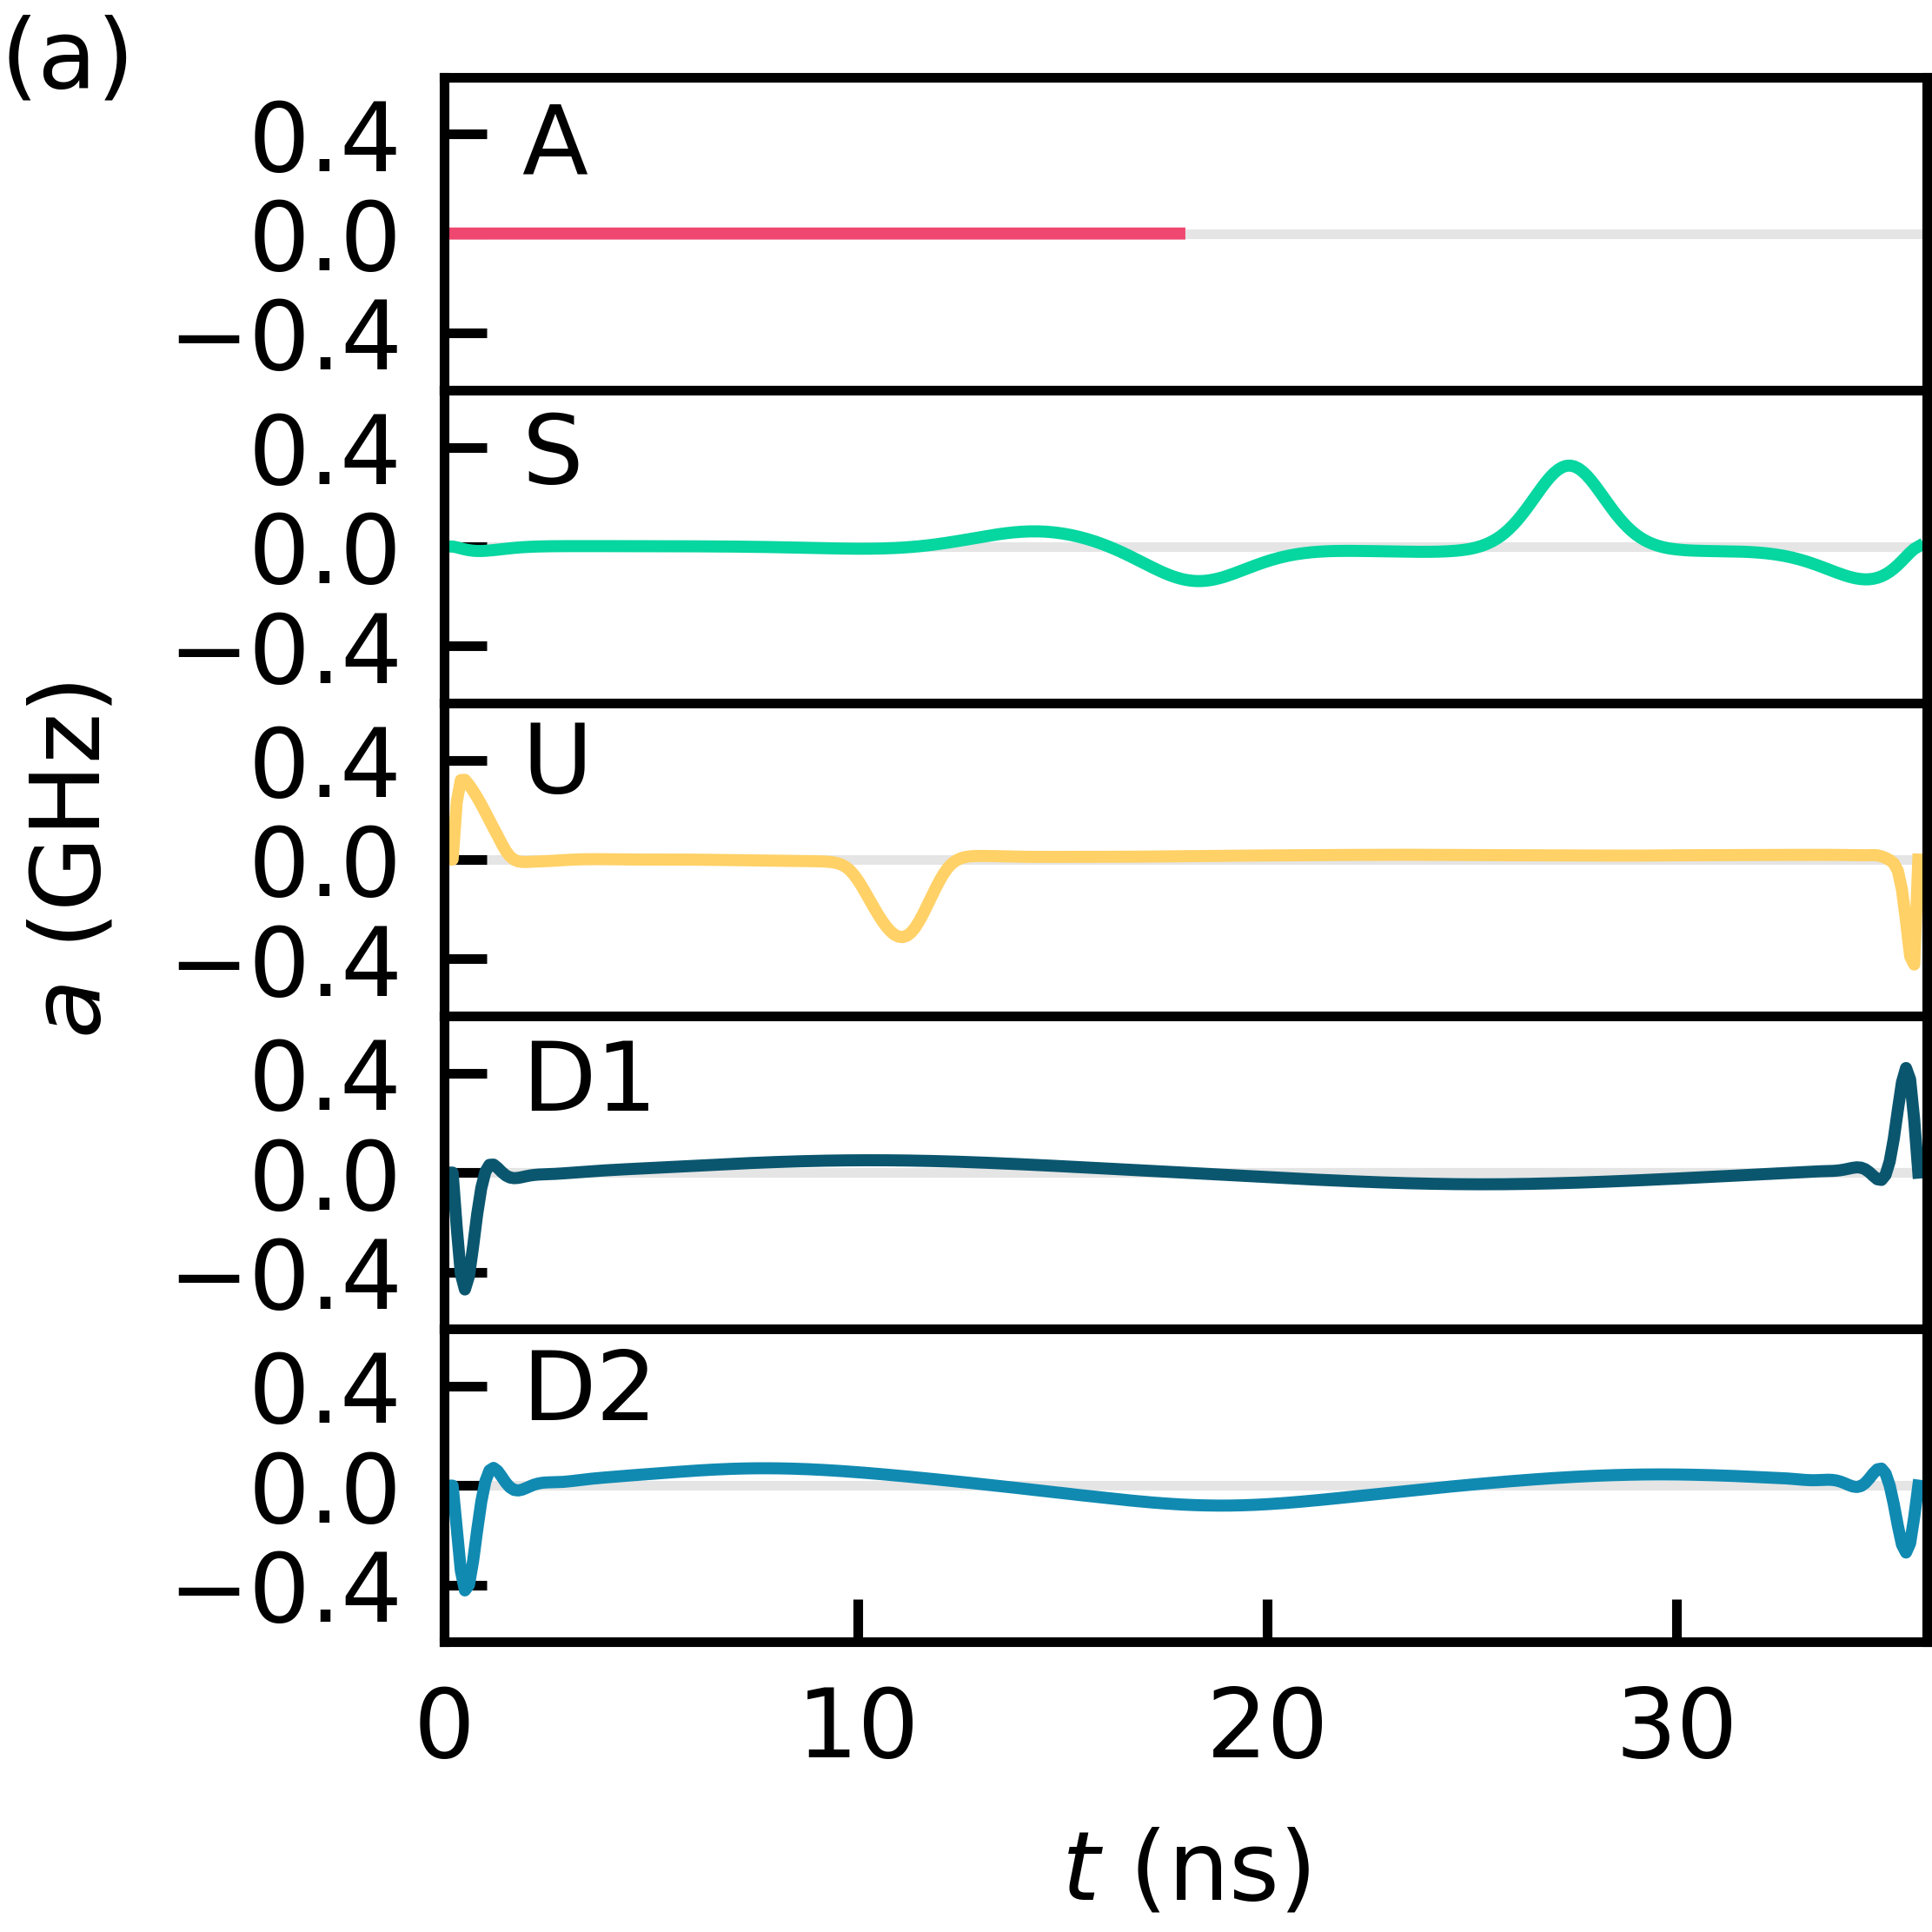
\includegraphics[width=\linewidth]{assets/f2a.png}
    \caption{\label{fig:statica}}
  \end{subfigure}\hfill
  \begin{subfigure}{.4\textwidth}
    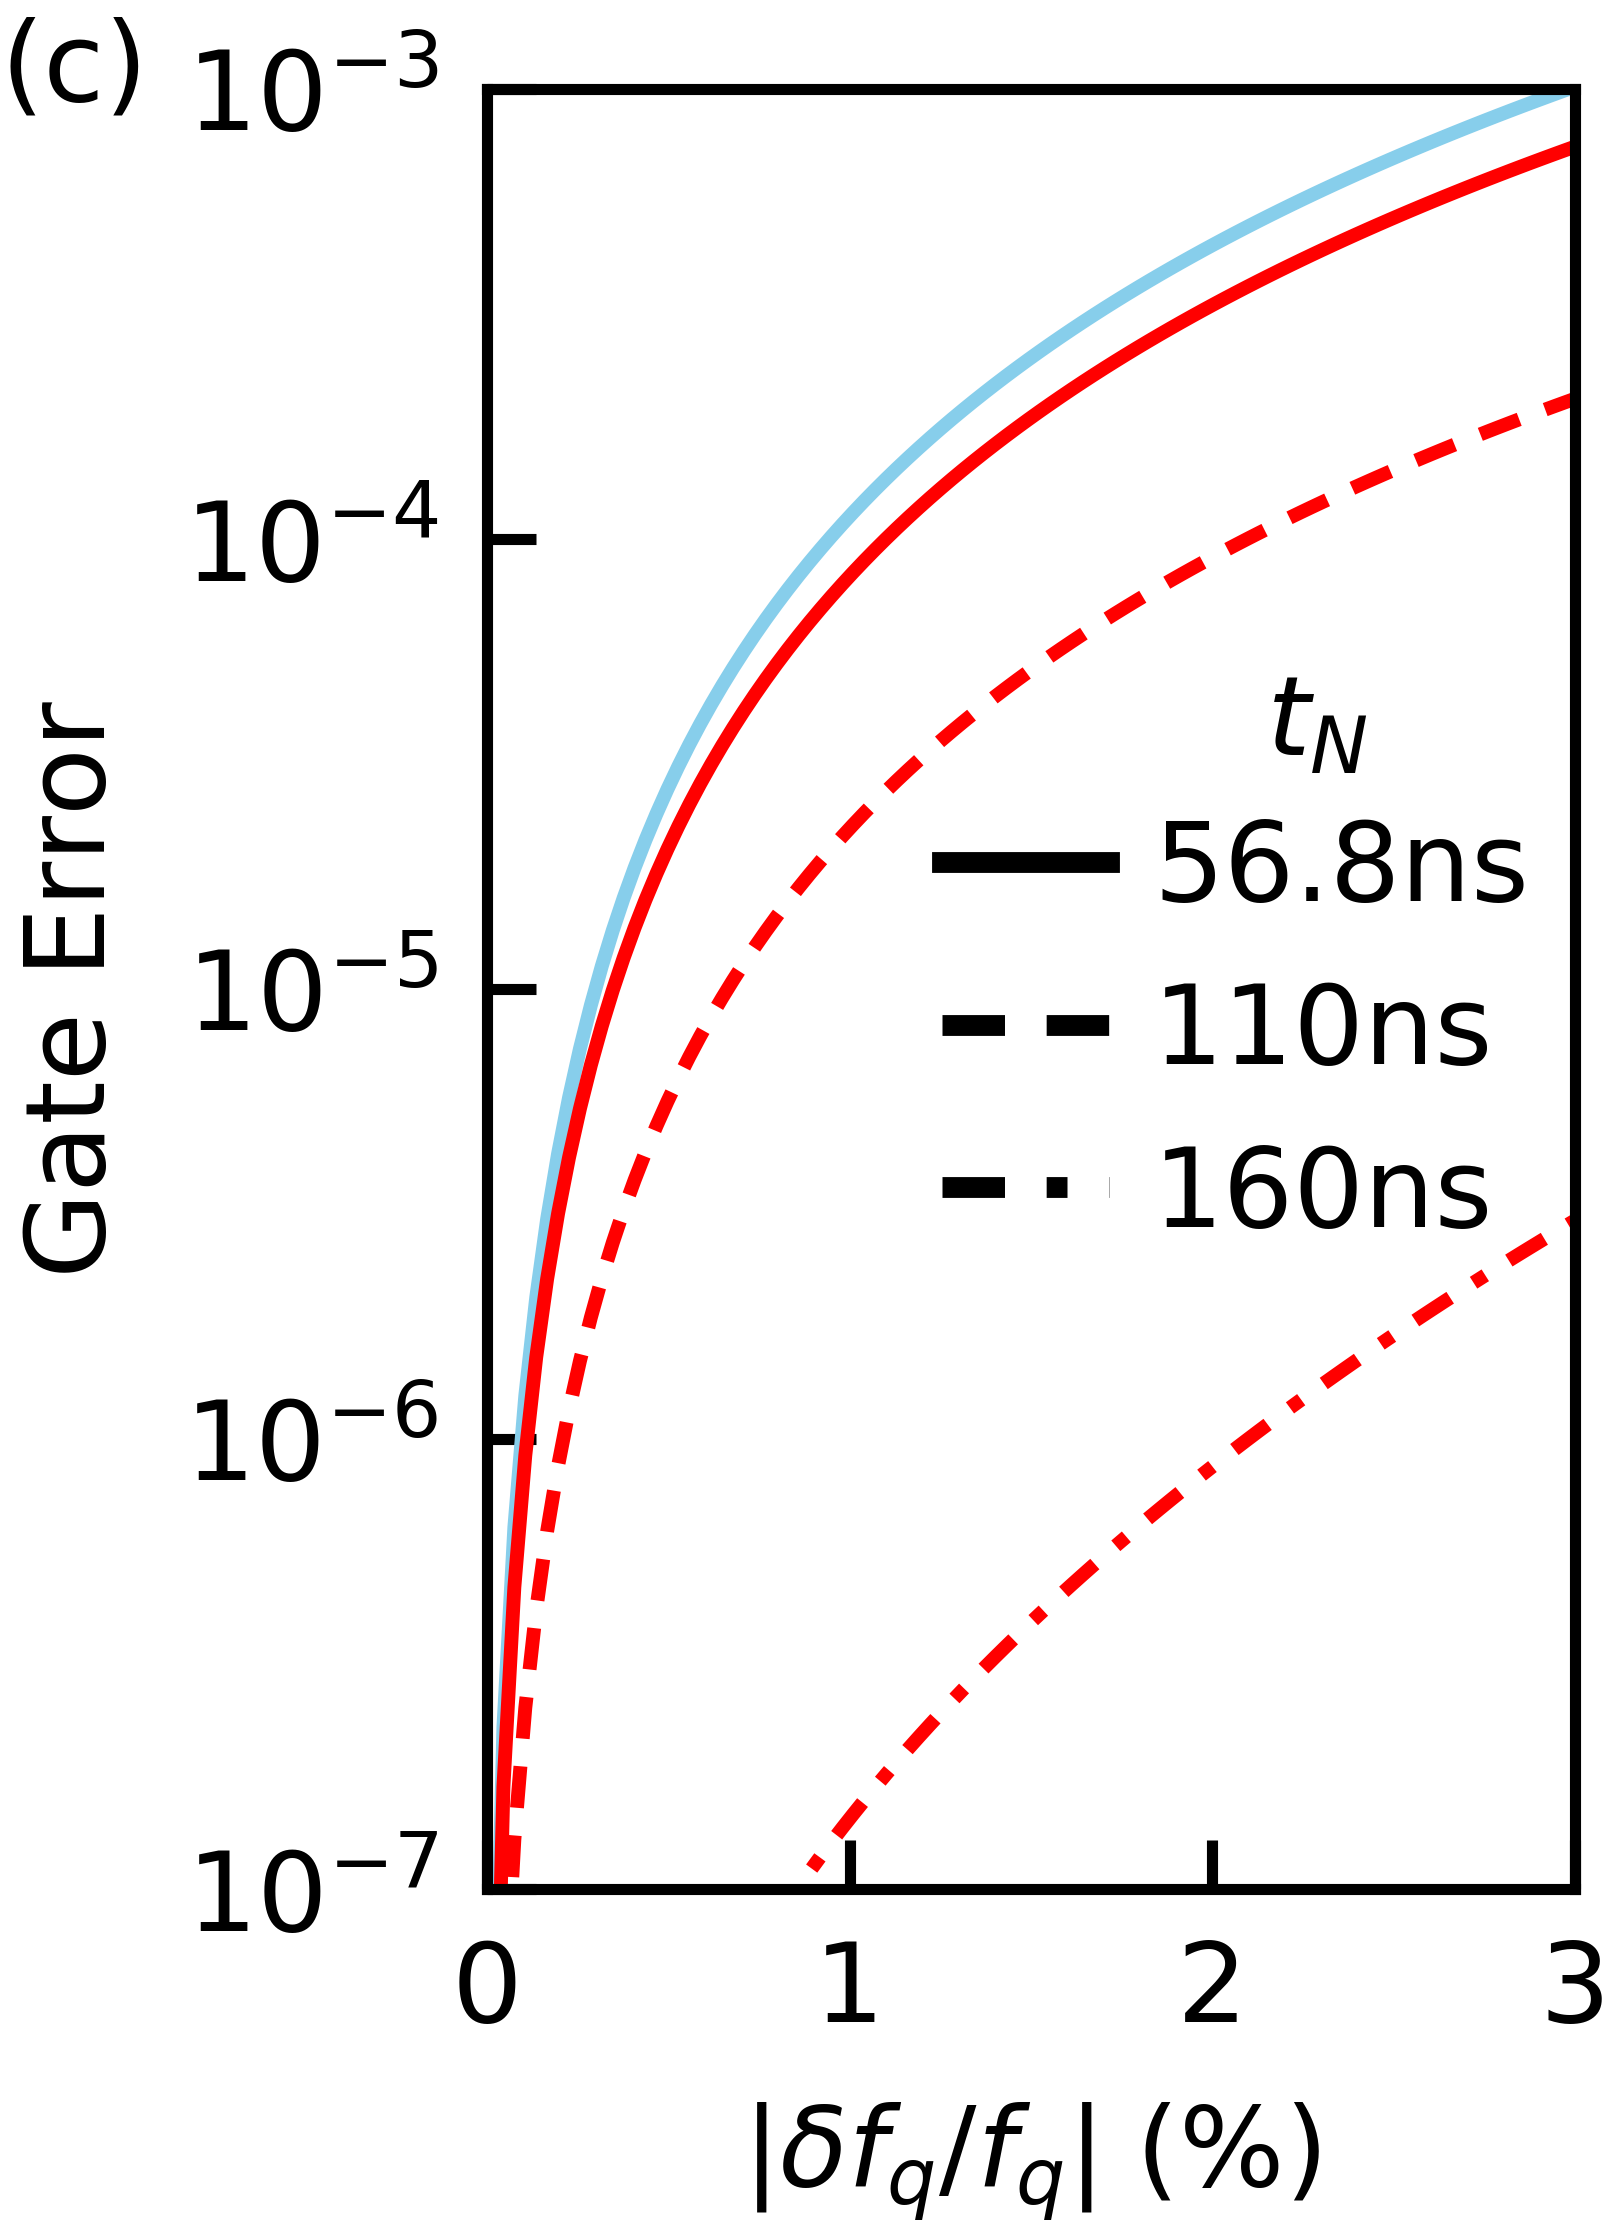
\includegraphics[width=\linewidth]{assets/f2b.png}
    \caption{\label{fig:staticb}}
  \end{subfigure}\hfill
  \begin{subfigure}{.23\textwidth}
    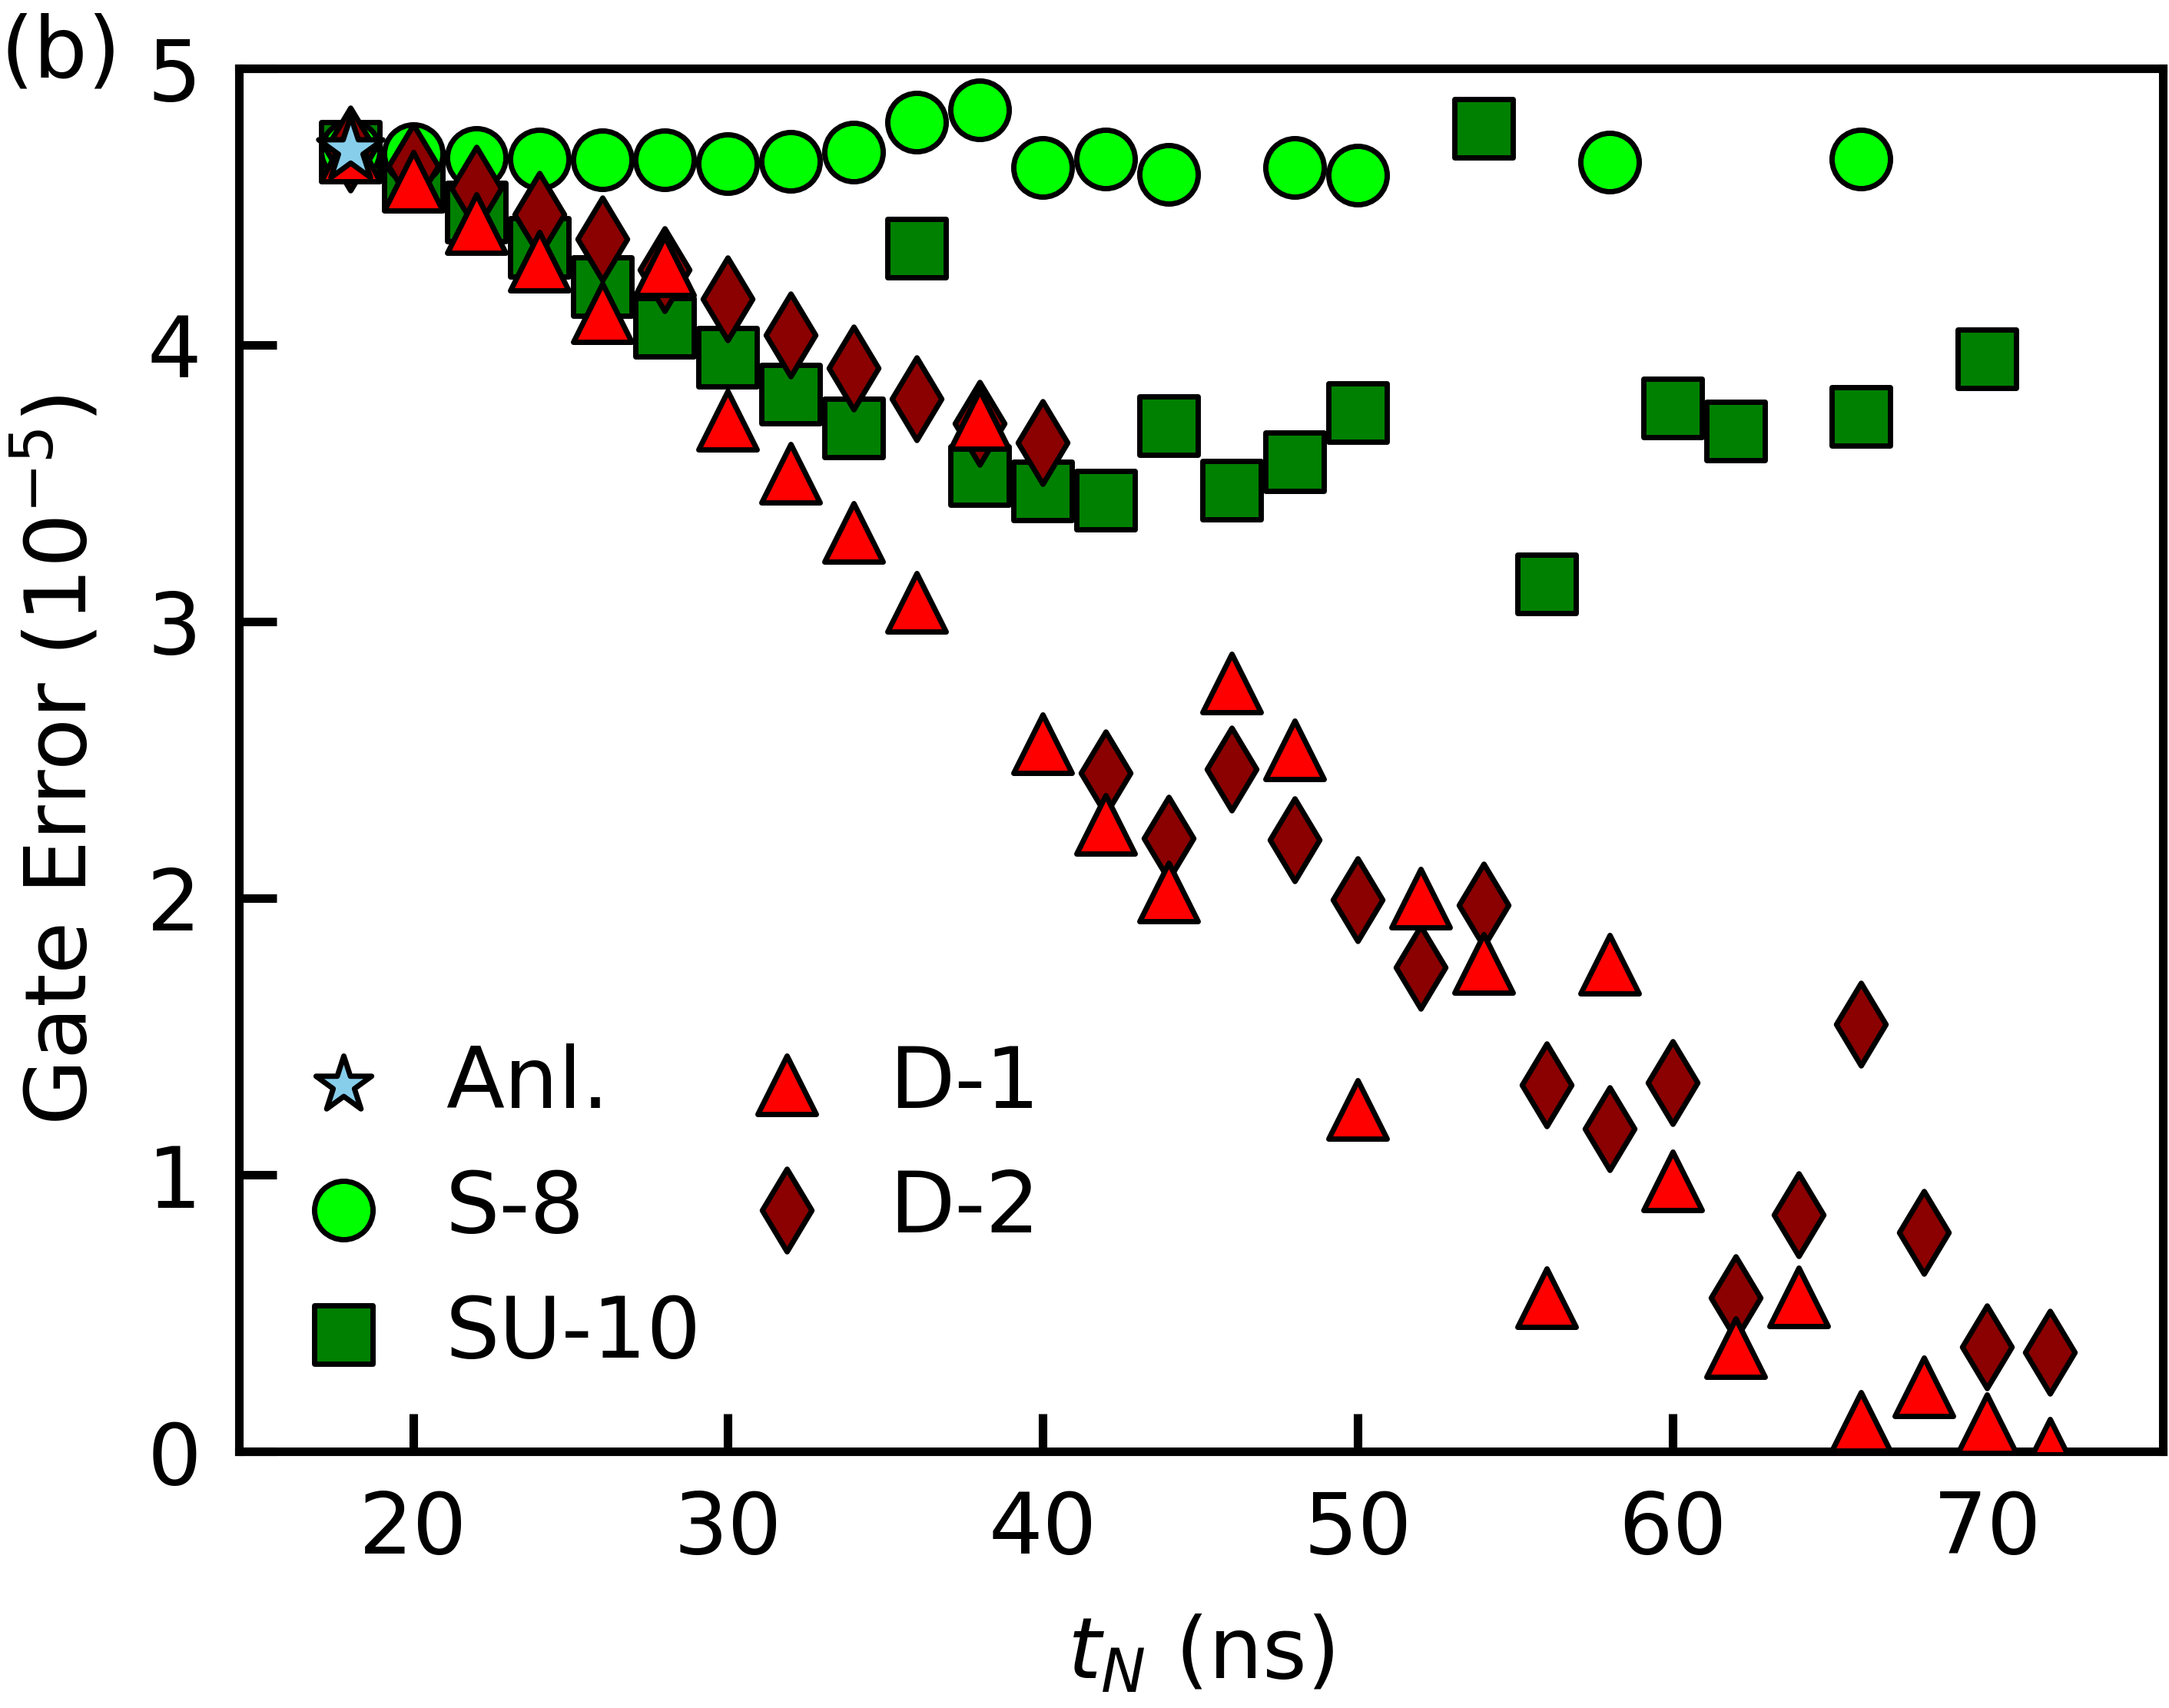
\includegraphics[width=\linewidth]{assets/f2c.png}
    \caption{\label{fig:staticc}}
  \end{subfigure}
  \caption{
    (a) $Z/2$ gates robust to qubit frequency detunings constructed with the
    analytic (A), sampling (S), unscented sampling (SU), and the 1\textsuperscript{st}-
    and 2\textsuperscript{nd}-order derivative methods (D1, D2). The numerical gates shown
    are optimized for twice the gate time of the analytic gate.
    (b) Single gate error at a one-percent qubit frequency detuning as
    a function of the gate time. Missing
    data points represent solutions with a gate error greater than $5 \cdot 10^{-5}$.
    (c) Single gate error as a function of the qubit frequency detuning.
    The gate errors for the analytic and 1\textsuperscript{st}-order derivative
    methods are shown for gate times which are multiples of $1 / 4 f_{q} \sim 18 \textrm{ns}$.
    The performance of the two methods is
    indistinguishable at the gate time $18 \textrm{ns}$.
  }
  \label{fig:static}
\end{figure*}

\section{Robustness to Static Parameter Uncertainty \label{sec:static}}
We have formulated the QOC
problem as an open-loop optimization problem, equivalently,
we do not incorporate feedback from the experiment in optimization.
However, the device typically deviates from the Hamiltonian we use in optimization,
leading to poor experimental performance. We combat errors
of this form using robust control techniques,
making the state evolution insensitive
to Hamiltonian parameter uncertainty. As an example,
we mitigate errors arising from the drift and finite measurement
precision of the qubit frequency which modifies the fluxonium Hamiltonian
\eqref{eq:hamiltonian} by $f_{q} \gets f_{q} + \delta f_{q}$.
We consider three robust control techniques to accomplish this task:
the sampling method, the unscented sampling method,
and the derivative method.

The sampling method incentivizes the optimizer
to ensure multiple copies of a state, each of which evolves
with a distinct value of the uncertain parameter, achieve
the same state transfer. For each initial state,
we add two sample states $\ket{\psi^{\pm}}$
to the augmented state \eqref{eq:astatecontrols}, and the discrete dynamics
function \eqref{eq:dyn_con} is modified
so the sample states evolve under the fluxonium Hamiltonian \eqref{eq:hamiltonian}
with $f_{q} \gets f_{q} \pm \sigma_{f_{q}}$ for a fixed hyperparameter
$\sigma_{f_{q}}$ which is the standard deviation of the qubit frequency.
For this method, the standard orthonormal basis states are an insufficient choice
for the initial states. As an example, a $Z/2$ gate achieved by idling
at the flux frustration point $a_{k} = 0 \ \forall \ k$
will be robust to qubit frequency detunings for the initial states $\ket{0}$
or $\ket{1}$ because the fidelity metric is insensitive to global phases,
but this gate will not be robust for any other initial states.
Thus, we choose four initial states
so that their outer products
span the operators on the Hilbert space
$\{\ket{0}, \ket{1}, (\ket{0} + i\ket{1}) / \sqrt{2},
(\ket{0} - \ket{1}) / \sqrt{2}\}$ \cite{chow2009randomized}.
The infidelities between the sample states and the images of their
initial states under the desired gate are penalized
by adding a cost function
$\sum_{k, \pm} q_{k} (1 - {\lvert \braket{\psi^{\pm}_{k}}{U \psi^{\pm}_{1}} \rvert}^{2})$
to the objective \eqref{eq:costfun} for a constant $q_{k}$ we supply.

For the unscented sampling method, we append $2(2n + d)$ sample
states to the augmented state vector \eqref{eq:astatecontrols}
for each initial state used in the sampling method. $2n = 4$ is twice the
dimension of the Hilbert space, resulting from the isomorphism \eqref{eq:isomorphism},
and $d = 1$ is the number of uncertain parameters. The sample states
encode a unimodal distribution over the $2n$
elements of the evolving initial state, modeling
the uncertainty in the state due to the uncertainty in the parameter.
The discrete dynamics function \eqref{eq:dyn_con} is modified
so each sample state evolves under the fluxonium Hamiltonian
\eqref{eq:hamiltonian} where $f_{q} \gets f_{q} + \delta f_{q}$
and $\delta f_{q}$ is sampled at each knot point from a distribution
with fixed standard deviation $\sigma_{f_{q}}$.
After propagating the sample states to each knot point, we apply the unscented
transformation to the states, which
preserves the first and second moments of the distribution the states encode.
This procedure makes the unscented sampling method more resistant to sample
states collapsing towards the mean than in the sampling method.
We add a contribution to the objective \eqref{eq:costfun} for the infidelity
of the sample states and their target states
as in the sampling method.
A detailed procedure for the unscented transformation is given
in Appendix \ref{appendix:unscented}.

The derivative method penalizes the sensitivty of the state
to the uncertain parameter, which is encoded in the $l$\textsuperscript{th}-order
state derivative $\partial_{f_{q}}^{l} \ket{\psi}$. In the $m$\textsuperscript{th}-order
derivative method, we append all state derivatives of order $1, \dots, m$
to the augmented state vector \eqref{eq:astatecontrols}
for each initial state used in the sampling method.
We penalize the norms of the state derivatives
in the objective \eqref{eq:costfun} by setting the corresponding elements
of the final augmented state $x_{f}$ to $0$.
We could obtain the state derivatives at each knot point
with backward-mode differentiation.
In a naive automatic differentiation scheme,
the discrete dynamics function at knot points
$1, \dots, k - 1$ would be differentiated to obtain the state
derivative at knot point $k$, requiring
$O(N^{2})$ matrix multiplications. Instead, we 
employ forward-mode differentiation on the TDSE \eqref{eq:tdse}
to obtain coupled, first-order ODEs
which require $O(N)$ matrix multiplications to integrate.
For example, the dynamics for the $1$\textsuperscript{st}-order derivative method are:
\begin{align}
  i \hbar \frac{d}{dt} \ket{\psi} &= H \ket{\psi}\\
  i \hbar \frac{d}{dt} \ket{\partial_{f_{q}}\psi} &=
  H \ket{\partial_{f_{q}} \psi} +
  (\partial_{f_{q}} H) \ket{\psi}
  \label{eq:d1dyn}
\end{align}
We integrate the coupled ODEs with exponential
integrators, see Appendix \ref{appendix:derivative},
in the discrete dynamics function \eqref{eq:dyn_con}. For runtimes
and complexity analyses for the three robust control techniques,
consult Appendix \ref{appendix:time}.

We compare the gate errors due to a static qubit frequency
detuning for $Z/2$ gates obtained with the robust control techniques
and the analytic method.
To compute the gate error,
an initial state is evolved
under the fluxonium Hamiltonian \eqref{eq:hamiltonian}
two separate times with the transformations
$f_{q} \rightarrow f_{q} \pm \delta f_{q}$
at the stated qubit frequency detuning.
The reported gate error is the infidelity of
the evolved state and the target state averaged over
the two transformations and $1000$ initial states.
We set $\sigma_{f_{q}}/f_{q} = 1\%$
for the sampling and unscented sampling
methods.

The analytic gate corresponds to
idling at the flux frustration point $a_{k} = 0 \ \forall \ k$, see Figure
\ref{fig:statica}. Its gate time $1 / 4 f_{q} \sim 18\textrm{ns}$
is the shortest possible for a $Z/2$ gate on the device.
The gate's erroneous rotation angle
$\pi \delta f_{q} / 2 f_{q}$ is linear in the
qubit frequency detuning, resulting in a gate error that is quadratic
in the detuning.
At a one-percent
qubit frequency detuning ($\lvert \delta f_{q} \rvert / f_{q} = 1\%$),
the gate error is $\sim 4.5 \cdot 10^{-5}$,
which is sufficient for quantum error correction.
Although the gate performs well, the method used to derive
it can not be employed to achieve a $Z/2$ gate at gate times other than
$1 / 4 f_{q}$. The ability to perform
phase gates in any given time is critical
for multi-qubit experiments, where the qubits operate at different
frequencies $f_{q, i} \neq f_{q, j}$.
We can find solutions using the numerical methods at
all gate times above $18$ns, see Figure \ref{fig:staticb}.
These numerical methods offer an effective scheme for synchronizing
multi-qubit experiments.

The solution for the unscented sampling method combines idling periods
with fast ramps to the maximum amplitude, whereas that for the sampling method
does not reach high amplitudes.
The gate error at a one-percent qubit frequency detuning for the sampling method
does not improve substantially over the
range of gate times. Conversely, the gate error at a one-percent detuning
for the unscented sampling method decreases linearly in the gate time
until half the Larmor period $1 / 2 f_{q}$ after which it has a consistent
gate error $\sim 3.5 \cdot 10^{-5}$.

The derivative methods converge on qualitatively similar solutions that
use fast triangle pulses at the boundaries and idle at low amplitudes.
The gate errors at a one-percent qubit frequency detuning
for both methods decrease super-linearly in their gate times.
The 1\textsuperscript{st}-order derivative method
consistently achieves lower gate errors than the
2\textsuperscript{nd}-order derivative method,
which we believe is related to the greater importance
of minimizing the 1\textsuperscript{st}-order state
derivative norm than the 2\textsuperscript{nd}-order
state derivative norm for this problem, see Appendix \ref{appendix:derivative}.
The gate error at a one-percent detuning for the 1\textsuperscript{st}-order
derivative method approaches zero at the Larmor period $1 / f_{q}$, see Figure \ref{fig:staticc}.
This result mimics the
ability of composite pulses to mitigate parameter uncertainty errors to arbitrary
order with sufficiently many pulses \cite{merrill2014progress}.
It is difficult to choose an appropriate composite pulse
for the problem studied here due to our Hamiltonian and experimental constraints.
We propose comparisons between composite pulses and numerical techniques
for future work.

%% F3
\begin{figure*}[ht]
  \begin{subfigure}{.4\textwidth}
    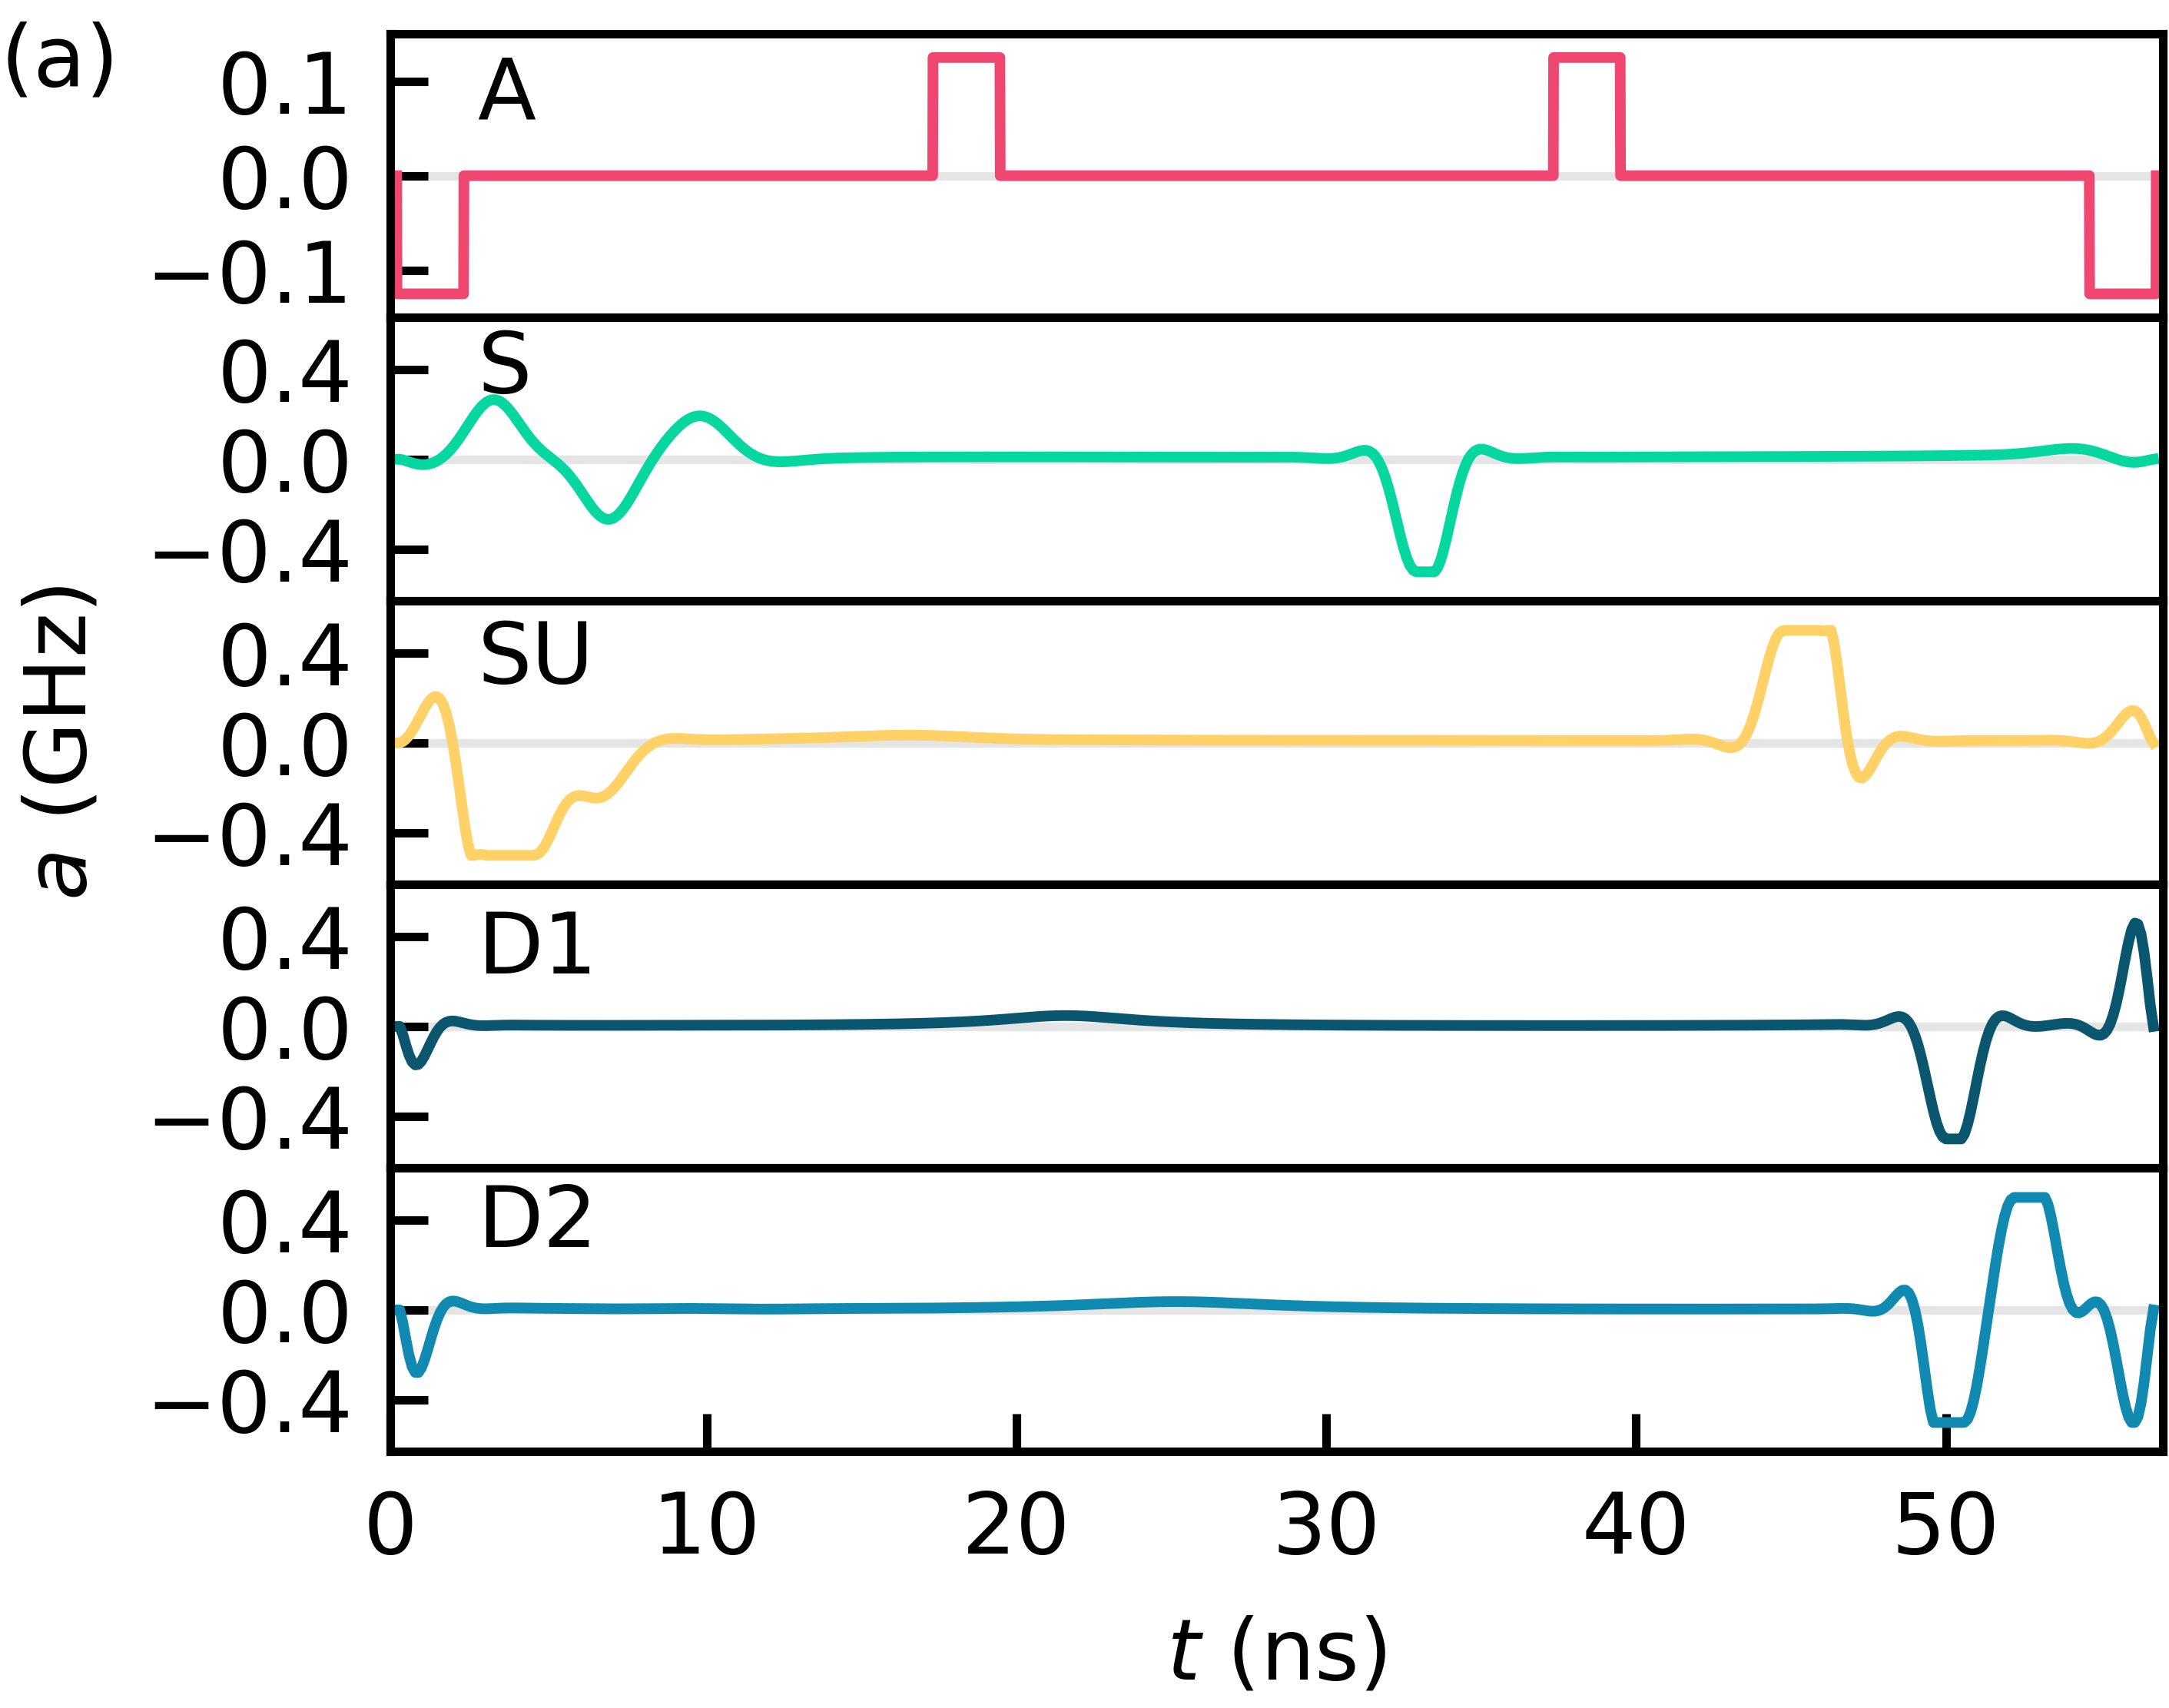
\includegraphics[width=\linewidth]{assets/f3a.png}
    \caption{}
    \label{fig:stochastica}
  \end{subfigure}\hspace{0.05\textwidth}
  \begin{subfigure}{.4\textwidth}
    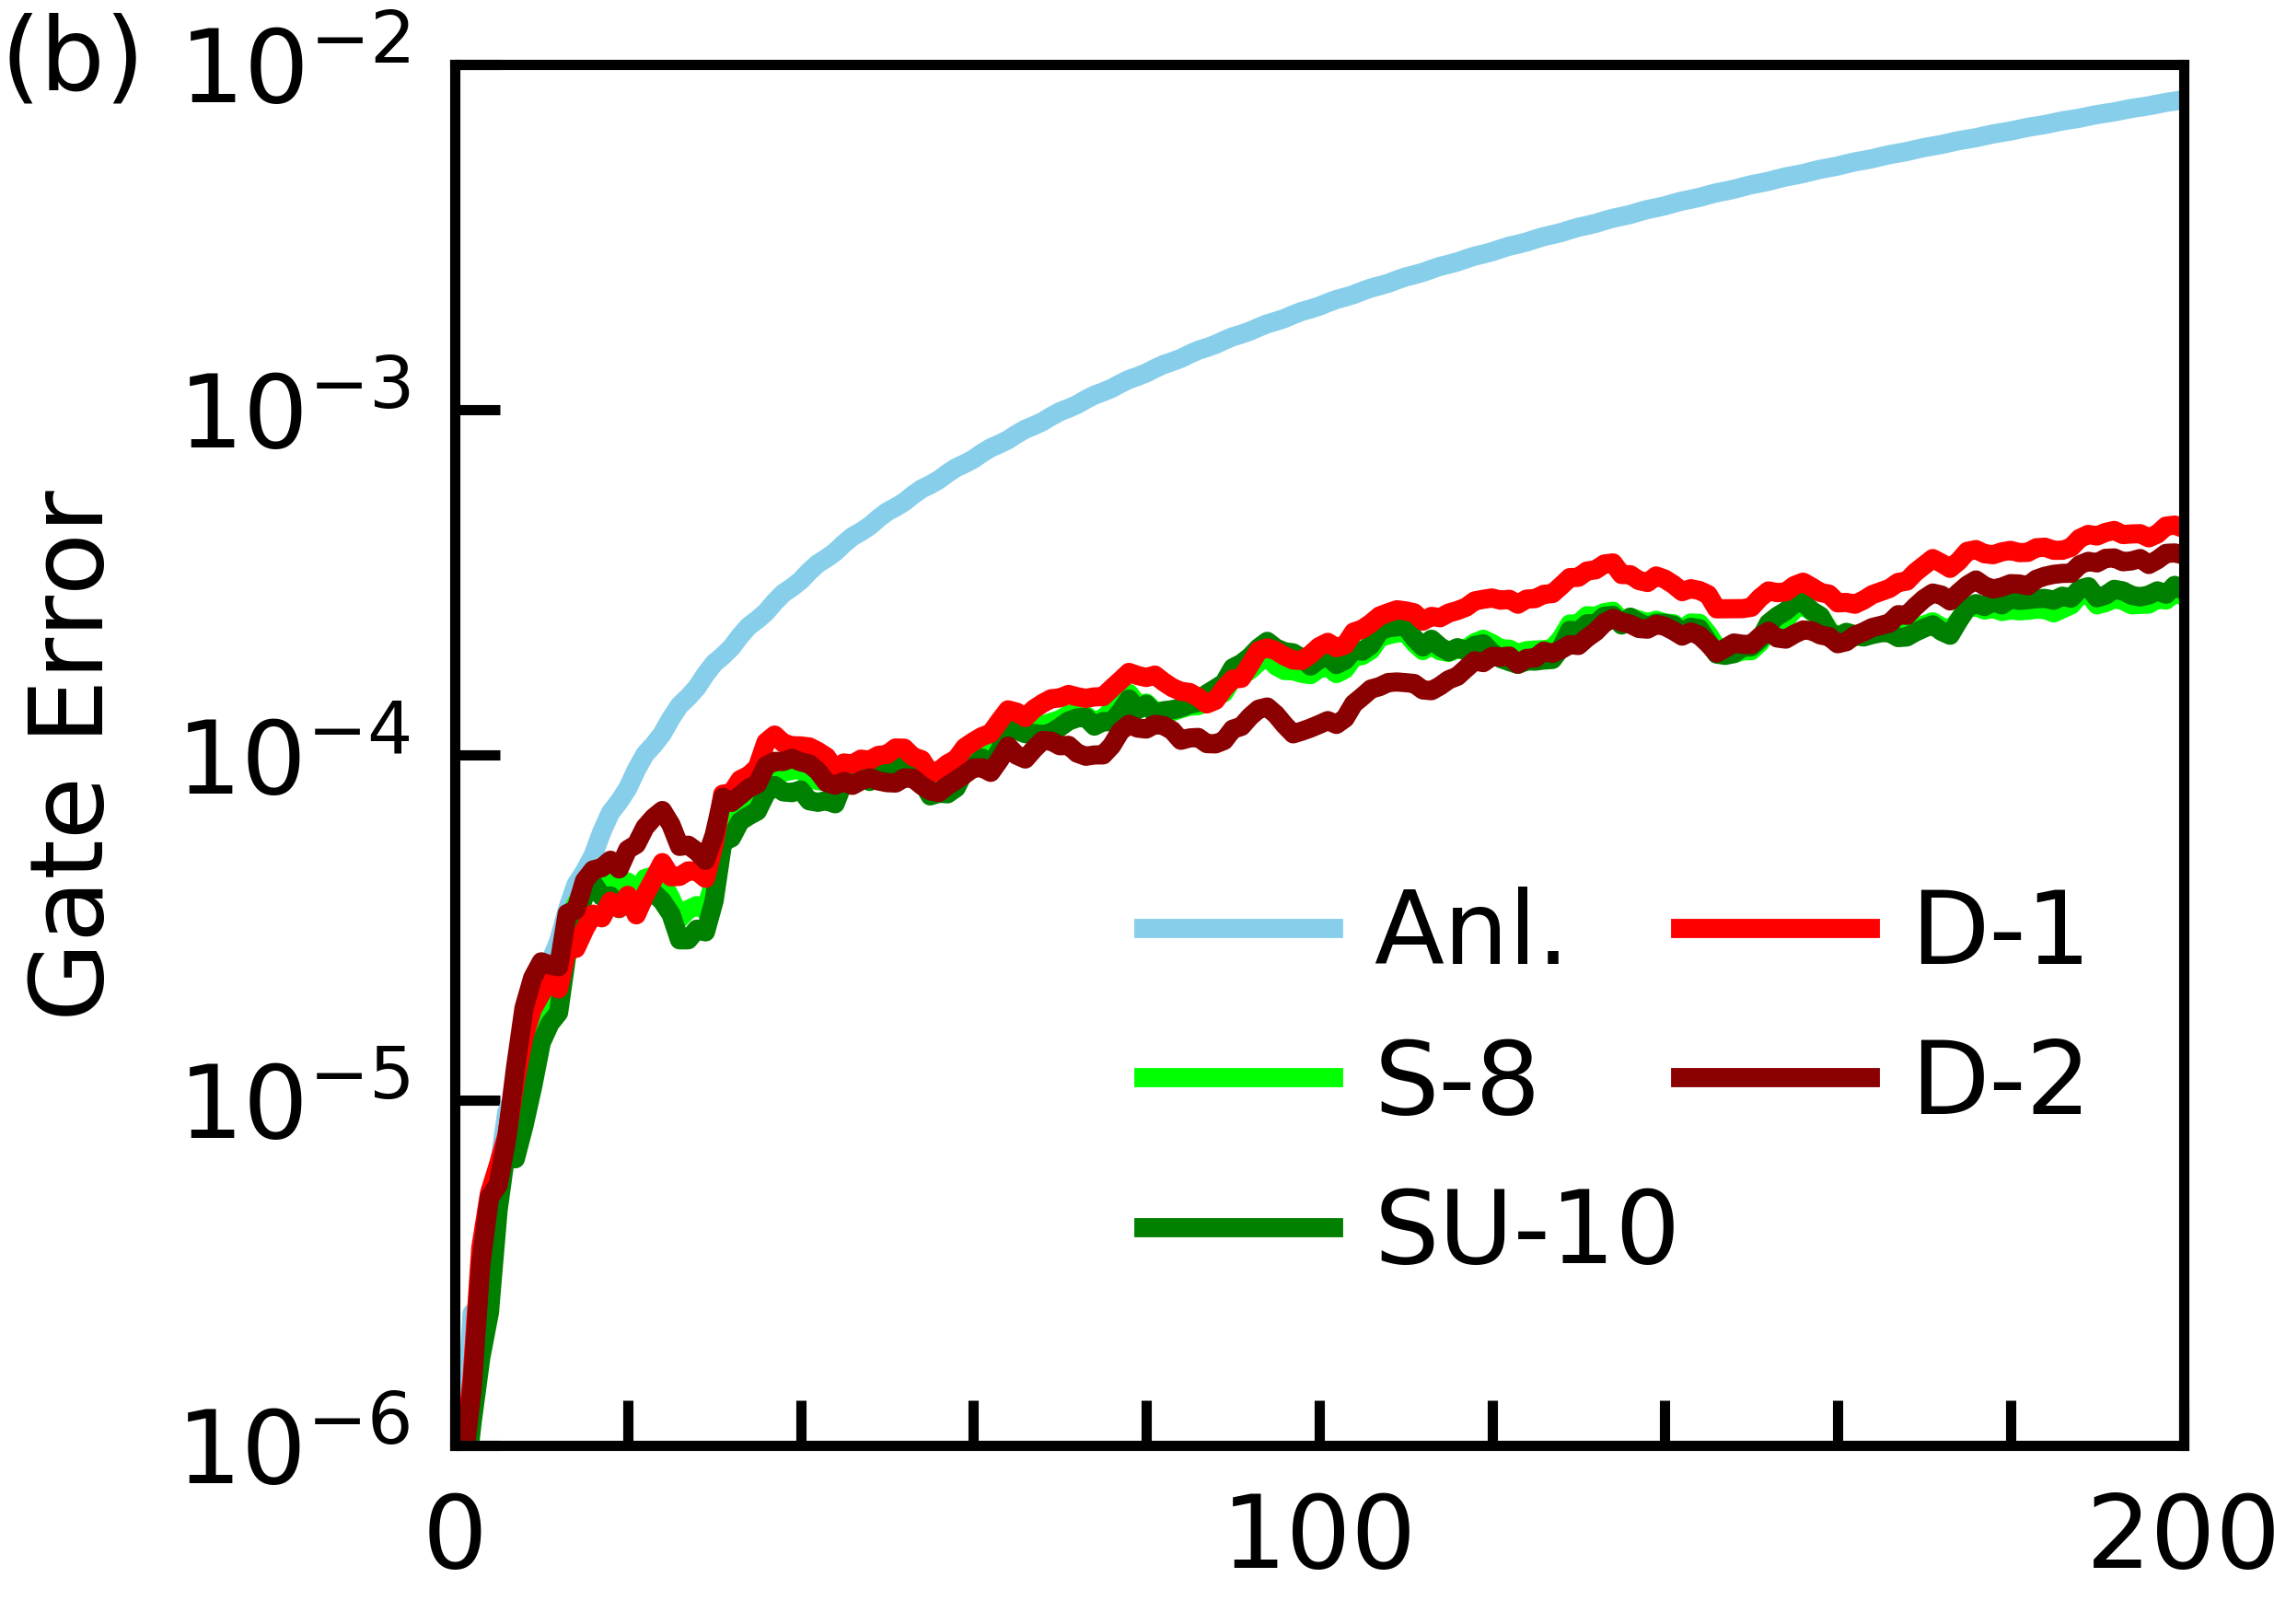
\includegraphics[width=\linewidth]{assets/f3b.png}
        \caption{}
    \label{fig:stochasticb}
  \end{subfigure}
  \caption{
    (a) $X/2$ gates robust to flux amplitude offsets constructed with the analytic (A),
    sampling (S), unscented sampling (SU), and the 1\textsuperscript{st}-
    and 2\textsuperscript{nd}-order derivative methods (D1, D2).
    (b) Cumulative gate error due to 1/$f$ flux noise for
    successive gate applications.
  }
  \label{fig:stochastic}
\end{figure*}
